\section{Reservoir ComputingとしてのRecurrent SNNの教師あり学習}
この章ではReservoir ComputingとしてのRecurrent SNNと、それを学習するためのFORCE法について解説します。
\section{Reservoir Computing}
\textbf{Reservoir Computing}は、RNN\footnote{ここでは発火率モデルについてのRNNについて述べています。}のモデルの一種です。一般のRNNが全ての結合重みを学習するのに対し、Reservoir ComputingではRNNのユニット間の結合重みはランダムに初期化して固定し、\textbf{出力の結合重みだけを学習}します。そのため、Reservoir Computingは学習するパラメータが少なく、学習も高速に行えます(もちろん関数の表現力は一般のRNNの方が優れています)。\par
Reservoirというのは溜め池(貯水池)を意味します。Reservoir Computingでは、まず入力信号をランダムな固定重みにより高次空間の信号に変換し、Reservoir RNN(信号の溜め池)に保持します。そして、Reservoir RNNのユニットの活動として保持された情報を学習可能な重みにより線形変換し、出力とします。このとき、ネットワークの出力が教師信号と一致するように出力重みを更新します。

%\begin{comment}
\begin{figure}[htbp]
    \centering
    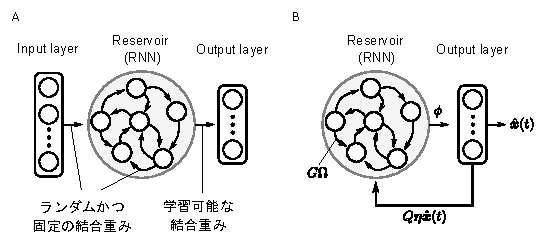
\includegraphics[scale=1.2]{figs/reservoir_computing.pdf}
    \caption{(A)Reservoir Computingの一般的なモデル。入力と中間にはランダムに固定された重みを用い、出力のみ学習可能となっています。 (B)FORCE法で用いるモデルの1つ。7.3節以降でこのモデルの実装を行います。}
    \label{fig:RC}
\end{figure}
%\end{comment}
